\documentclass{article}
\usepackage{graphicx}
\usepackage{tabu}
\usepackage[margin=3.0cm]{geometry}

\begin{document}
\begin{titlepage}
    \begin{center}
        \vspace*{1cm}
        \huge COMS3002 Software Engineering \\
        \LARGE Lab 2
        
		\vspace{1.5cm}        
		
		
\includegraphics[scale=0.5]{witsLogo.png} \\		
		\vspace{1.5cm}
        \textbf{Group 8} \\
        \large Abdulkadir Dere - 752817\\
        Jesse Wright - 721386 \\
        Liam Leibrandt - 814078\\
        Brenda Lin - 747243 \\
        
		\vspace{1.5cm} 
		       
                
        School of Computer Science\\
        University of Witwatersrand\\
        27 August 2017
        
    \end{center}
\end{titlepage}

\section*{Choice of a Software Development Life-Cycle}
\subsection*{SCRUM}
SCRUM is our choice of a software development life-cycle for our project. It is an agile development method which is iterative and incremental.
This is how we plan to implement it:
\begin{itemize}
\item We will create a wish list of use cases and add them to our backlog.
\item During sprint planning, we will pull some of the use cases from the backlog and add them to our sprint backlog, and then decide how to implement those use cases.
Our sprint time is 2 - 3 weeks, depending on the team's availability. 
\item Along the way, the ScrumMaster (Project Leader) keeps the team focused on its goal.
\item At the end of the sprint, the use cases should be implemented and work to the best of its ability. 
\item The sprint ends with a sprint review and retrospective.
As the next sprint begins, we will choose more use cases from the backlog and begin working again. \cite{Scrum}
\end{itemize}
\hfill

\section*{Choice of Architecture}
\subsection*{Three Tier Architecture}
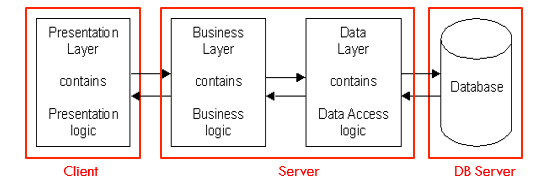
\includegraphics[scale=1]{Capture2.png} 
\begin{itemize}
\item A Presentation Layer that sends content to browsers in the form of HTML/JS/CSS. 
\item An Application Layer that uses an application server and processes the business logic for the application. This might be written in C\# or JavaScript.
\item A Data Layer which is a database management system that provides access to application data. This could be SQL Server or Azure. \\
\end{itemize}

\subsection*{Benefits}
\begin{itemize}
\item It gives you the ability to update the technology stack of one tier, without impacting other areas of the application.
It allows for team members to each work on their own areas of expertise.
\item You are able to scale the application up and out. A separate back-end tier, for example, allows you to deploy to a variety of databases instead of being locked into one particular technology. It also allows you to scale up by adding multiple web servers.
\item It adds reliability and more independence of the underlying servers or services.
\item It provides an ease of maintenance of the code base, managing presentation code and business logic separately, so that a change to business logic, for example, does not impact the presentation layer. \cite{tier}
\end{itemize}

\section*{Front-end Interface Method}
A web application which allows for browser support will be created. There it should work on most browsers including mobile browsers.

\section*{Back-End Service}
ASP.net MVC uses SQL Server and we will use a cloud service such as Azure or Amazon web services.

\section*{Other Supporting Software}
Dot Net Highcharts will be used for any reporting functionality we might have.Bootstrap will also be used to make sure that the web app looks good and works on all browsers. \\

\begin{thebibliography}{9}
\bibitem{Scrum}
Scrum Alliance, \\
\texttt{https://www.scrumalliance.org/why-scrum}

\bibitem{tier}
Bob Pepalis, IZENDA, \\
\texttt{https://www.izenda.com/blog/5-benefits-3-tier-architecture/}

\end{thebibliography}

\end{document}